\documentclass[xcolor={svgnames},
               hyperref={colorlinks,citecolor=DeepPink4,linkcolor=FireBrick,urlcolor=Maroon}]
               {beamer}

\mode<presentation>{
  \usetheme{Madrid}
  \usecolortheme{seagull}
  \setbeamercovered{transparent}
  \setbeamerfont{frametitle}{size=\large}
}

\setbeamercolor*{block title}{bg=red!10}
\setbeamercolor*{block body}{bg=red!5}

\usepackage[english]{babel}
\usepackage[latin1]{inputenc}
\usepackage{times}
\usepackage[T1]{fontenc}
% Or whatever. Note that the encoding and the font should match. If T1
% does not look nice, try deleting the line with the fontenc.

\usepackage{empheq,bm}
\usepackage{xspace}
\usepackage{fancyvrb}

\usepackage{tikz}
\usetikzlibrary{shapes,arrows.meta,decorations.markings,decorations.pathreplacing,fadings,positioning}

\usepackage[kw]{pseudo}
\pseudoset{left-margin=15mm,topsep=5mm,idfont=\texttt,st-left=,st-right=}


% If you wish to uncover everything in a step-wise fashion, uncomment
% the following command:
%\beamerdefaultoverlayspecification{<+->}

\newcommand{\ba}{\mathbf{a}}
\newcommand{\bb}{\mathbf{b}}
\newcommand{\bc}{\mathbf{c}}
\newcommand{\bbf}{\mathbf{f}}
\newcommand{\bg}{\mathbf{g}}
\newcommand{\bn}{\mathbf{n}}
\newcommand{\bq}{\mathbf{q}}
\newcommand{\br}{\mathbf{r}}
\newcommand{\bx}{\mathbf{x}}
\newcommand{\by}{\mathbf{y}}
\newcommand{\bv}{\mathbf{v}}
\newcommand{\bu}{\mathbf{u}}
\newcommand{\bw}{\mathbf{w}}

\newcommand{\bF}{\mathbf{F}}
\newcommand{\bG}{\mathbf{G}}
\newcommand{\bQ}{\mathbf{Q}}

\newcommand{\grad}{\nabla}
\newcommand{\Div}{\nabla\cdot}

\newcommand{\argmin}{\operatorname{argmin}}

\newcommand{\CC}{\mathbb{C}}
\newcommand{\EE}{\mathbb{E}}
\newcommand{\RR}{\mathbb{R}}

\newcommand{\ddt}[1]{\ensuremath{\frac{\partial #1}{\partial t}}}
\newcommand{\ddx}[1]{\ensuremath{\frac{\partial #1}{\partial x}}}
\newcommand{\Matlab}{\textsc{Matlab}\xspace}
\newcommand{\Octave}{\textsc{Octave}\xspace}
\newcommand{\eps}{\epsilon}

\newcommand{\ip}[2]{\left<#1,#2\right>}

\newcommand{\xiphalf}{{x_{i+\frac{1}{2}}}}
\newcommand{\ximhalf}{{x_{i-\frac{1}{2}}}}
\newcommand{\Fiphalf}{{F_{i+\frac{1}{2}}}}
\newcommand{\Fimhalf}{{F_{i-\frac{1}{2}}}}
\newcommand{\Fiphalfn}{{F^n_{i+\frac{1}{2}}}}
\newcommand{\Fimhalfn}{{F^n_{i-\frac{1}{2}}}}

\newcommand{\trefcolumn}[1]{\begin{bmatrix} \phantom{x} \\ #1 \\ \phantom{x} \end{bmatrix}}
\newcommand{\trefmatrixtwo}[2]{\left[\begin{array}{c|c|c} & & \\ #1 & \dots & #2 \\ & & \end{array}\right]}
\newcommand{\trefmatrixthree}[3]{\left[\begin{array}{c|c|c|c} & & & \\ #1 & #2 & \dots & #3 \\ & & & \end{array}\right]}
\newcommand{\trefmatrixgroups}[4]{\left[\begin{array}{c|c|c|c|c|c} & & & & & \\ #1 & \dots & #2 & #3 & \dots & #4 \\ & & & & & \end{array}\right]}

\newcommand{\blocktwo}[4]{\left[\begin{array}{c|c} #1 & #2 \\ \hline #3 & #4 \end{array}\right]}

\newcommand{\bqed}{{\color{blue}\qed}}
\newcommand{\ds}{\displaystyle}

\newcommand\mynum[1]{{\renewcommand{\insertenumlabel}{#1}%
      \usebeamertemplate{enumerate item} \,}}


\title{Online optimization}

\subtitle{\emph{ML training algorithms regret less}}

\author{Ed Bueler}

\institute[UAF]{MATH 692 Mathematics for Machine Learning}

\date[]{17 March 2022}

%\titlegraphic{\begin{picture}(0,0)
%    \put(0,180){\makebox(0,0)[rt]{\includegraphics[width=4cm]{figs/software.png}}}
%  \end{picture}
%}

%% to start section counter at 0 see
%% https://tex.stackexchange.com/questions/170222/change-the-numbering-in-beamers-table-of-content


\begin{document}
\beamertemplatenavigationsymbolsempty

\begin{frame}
  \maketitle
\end{frame}


\begin{frame}{Outline}
  \tableofcontents[hideallsubsections]
\end{frame}


\begin{frame}{my motivations}

\begin{itemize}
\item why is SGD so popular? is my algorithm better than yours?

\medskip
\item it was easy to stumble upon:

\medskip
\begin{center}
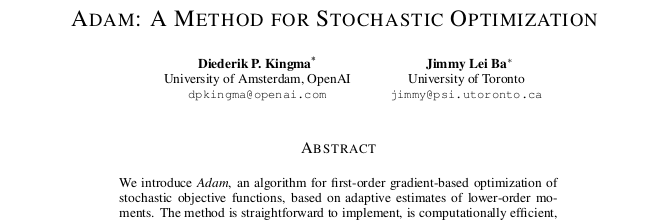
\includegraphics[width=0.7\textwidth]{figs/adam-paper.png}
\end{center}

\medskip
    \begin{itemize}
    \item[$-$] 100651 citations
    \item[$-$] the Adam optimizer is the default for \href{https://www.tensorflow.org/tutorials/keras/classification}{tensorflow}, \href{https://pytorch.org/docs/stable/optim.html}{pytorch}, \dots
    \end{itemize}

\medskip
\item so, how do they analyze Adam and show that it is good?
\end{itemize}
\end{frame}


\section{online optimization framework}

\begin{frame}{training a neural net (connecting to my earlier talk)}

\begin{itemize}
\item forward pass through an artificial neural net (ANN) with $L$ layers:

\begin{columns}
\begin{column}{0.1\textwidth}
$x^{\{i\}}\to$ 
\end{column}
\begin{column}{0.4\textwidth}
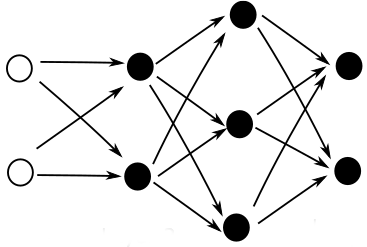
\includegraphics[height=30mm]{figs/cleannet.png}
\end{column}
\begin{column}{0.45\textwidth}
$\to a^{[L]}$ \hfill (supposed to be $y^{\{i\}}$)
\end{column}
\end{columns}

\item output activations are a function of input and parameters:
    $$a^{[L]} = a^{[L]}(x^{\{i\}}; p)$$
\item parameters $p$ collect weights and biases:
    $$p=\{W^{[2]},\dots,W^{[L]},b^{[2]},\dots,b^{[L]}\} \in \RR^n$$
\item cost of one labeled pair $(x^{\{i\}},y^{\{i\}})$:
    $$C^{\{i\}}(p) = \frac{1}{2} \left\|y^{\{i\}} - a^{[L]}(x^{\{i\}}; p)\right\|_2^2$$
\end{itemize}
\end{frame}


\begin{frame}{notation (standardization and simplification)}

\begin{itemize}
\item $\theta = p$ is vector of parameters
\item $(x_i,y_i) = (x^{\{i\}},y^{\{i\}})$ is a labeled pair
\item $N$ is total size of training set
\item $c_i(\theta) = \frac{1}{2} \left\|y_i - a^{[L]}(x_i; \theta)\right\|_2^2 = C^{\{i\}}(p)$ is cost of one pair
\end{itemize}
\end{frame}


\begin{frame}{total cost versus online cost sequence}

\begin{block}{total cost of training set}
original goal:  minimize total (average) cost over fixed training set
    $$\frac{1}{N} \sum_{i=1}^N c_i(\theta)$$
\end{block}

\begin{block}{online training $=$ sequence of cost objectives}
assume infinite sequence of cost functionals:
    $$c_i(\theta)$$
\end{block}

\begin{itemize}
\item the basic online training \textbf{method} is clear: train the neural net incrementally, a little for each $c_i$
\item but what's the online training \textbf{goal}?
\end{itemize}

\end{frame}


\begin{frame}{online training algorithms}

\begin{itemize}
\item somehow choose $\theta_1$ as the initial iterate for the parameters
\item an \emph{online training algorithm} computes each new iterate $\theta_{i+1}$
\item $\theta_{i+1}$ is computed from previous cost functionals $\{c_1,c_2,\dots,c_i\}$ and (parameter) iterates $\{\theta_1,\theta_2,\dots,\theta_i\}$
\item \textbf{key assumption:} an online  training algorithm does not use \emph{future} cost functionals in constructing $\theta_{i+1}$:
    $$\theta_{i+1} = F(c_1,\dots,c_i,\theta_1,\dots,\theta_i)$$
\end{itemize}
\end{frame}


\begin{frame}{online training algorithm examples}

\begin{itemize}
\item \emph{online gradient descent} (OGD) with learning rates $\eta_i$:
   $$\theta_{i+1} = \theta_i - \eta_i \grad c_i(\theta_i)$$

    \begin{itemize}
    \item[$\circ$] probability is not needed so jettison ``stochastic'': SGD $\to$ OGD
    \end{itemize}
\item Adam (\emph{more later})
\item Adaline, Adadelta, Adagrad, RMSprop, mini-batching, dropout, \dots
    \begin{itemize}
    \item[$\circ$] google search for buzzwords: \quad \texttt{tensorflow optimizers}
    \end{itemize}
\item (quasi-)Newton methods which use (approximate) 2nd derivatives
\end{itemize}
\end{frame}


\section{regret}

\begin{frame}{regret of an online algorithm}

\begin{block}{\textbf{definition} (Zinkevich, 2003; decision theory in 1980s?)}
the \emph{regret} of an online algorithm, at the $k$th training step, is
    $$R_j = \sum_{i=1}^j c_i(\theta_i) - \min_\theta \sum_{i=1}^j c_i(\theta)$$
\end{block}

\begin{itemize}
\item regret $R_j$ is difference between algorithm's result for the stream so far and the best-possible cost from a single parameter setting
    \begin{itemize}
    \item[$\circ$] best setting so far:\quad  $\ds \theta_j^* = \begin{smallmatrix} \phantom{x} \\ \text{\footnotesize argmin} \\ \theta \end{smallmatrix} \sum_{i=1}^j c_i(\theta)$
    \end{itemize}

\smallskip
\item $R_j>0$: the player regrets not choosing $\theta_j^*$
\item negative regret is possible!
\end{itemize}
\end{frame}


\begin{frame}{regret in game theory}

\begin{itemize}
\item treat the algorithm as a \emph{player} and the online stream of cost functionals $c_i$ as an \emph{adversary}
\item the player chooses $\theta_{i+1}$ \alert{before} knowing $c_{i+1}$
\item the adversarial sequence $\{c_i\}$ is totally uncontrolled
\end{itemize}

\begin{block}{online convex game (Abernathy et al 2008)}
\begin{pseudo*}
for $i = 0,1,\dots,j-1$ \\+
    \st{player chooses} $\theta_{i+1}$ \\
    \st{adversary chooses} $c_{i+1}$ \\-
\st{player suffers regret} \\+
    $\ds R_j = \sum_{i=1}^j c_i(\theta_i) - \min_\theta \sum_{i=1}^j c_i(\theta)$
\end{pseudo*}
\end{block}
\end{frame}


\begin{frame}{convex sets}

\begin{itemize}
\item previous slide says ``convex''; we need the definition
\end{itemize}

\begin{block}{definition}
\begin{itemize}
\item a set $K \subset \RR^n$ is \emph{convex} if for all $x,y \in K$ and $0 \le t \le 1$,
  $$t\, x + (1-t) y \in K$$

    \begin{itemize}
    \item[$\circ$] line segment from
    \item[]  $x$ to $y$ is inside $K$
    \end{itemize}

\vspace{-8mm}
\hfill 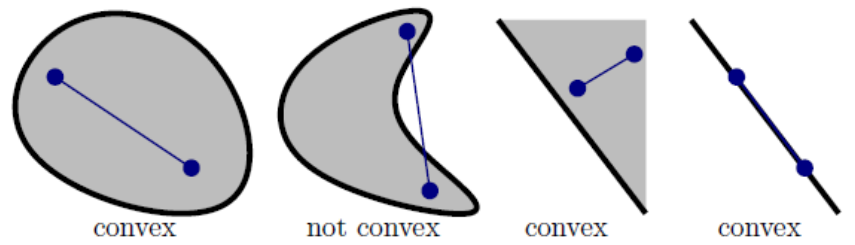
\includegraphics[width=0.6\textwidth]{figs/convex}
\end{itemize}
\end{block}
\end{frame}


\begin{frame}{convex functions}

\begin{itemize}
\item convex sets \emph{and} functions
\end{itemize}

\begin{block}{definition}
\begin{itemize}
\item a function $f:K \to \RR$ is \emph{convex} if for all $x,y \in K$ and $0 \le t \le 1$,
  $$t\, f(x) + (1-t) f(y) \ge f(t\, x + (1-t) y)$$
\end{itemize}
\end{block}

\begin{itemize}
\item for $f:K\to \RR$ to be convex, note $K$ must be convex
\item convex = concave \emph{up}
\end{itemize}
\end{frame}


\begin{frame}{convex optimization: a classical topic}

\begin{block}{definition}
given a convex set $K \subset \RR^n$ and a convex function $f:K\to \RR$,
    $$\min_{\theta \in K} f(\theta)$$
is a \emph{convex optimization problem}
\end{block}

\begin{itemize}
\item $K$ is often described by equality and inequality constraints
\item $K=\RR^n$ is convex (unconstrained optimization)
\item SVM is convex optimization, with nontrivial $K$
\item \emph{I don't know the answer}:

for an ANN, when is $C^{\{i\}}(\theta) = \frac{1}{2} \left\|y^{\{i\}} - a^{[L]}(x^{\{i\}}; \theta)\right\|_2^2$ a convex function on $K = \RR^n$?
\end{itemize}
\end{frame}


\begin{frame}{convex optimization: the default algorithm}

\begin{itemize}
\item to solve: \quad $\ds \min_{\theta \in K} f(\theta)$
\item assume $K\subset \RR^n$ is closed and convex
    \begin{itemize}
    \item[$-$] each $y\in \RR^n$ has a unique \emph{projection onto } $K$:
    $$\Pi_K(y) = \argmin_{x\in K} \|y - x\|_2$$
    \item[$-$] $\Pi_K(y)$ is the closest point in $K$ to $y$
    \end{itemize}
\item assume $f:K\to \RR$ is differentiable and convex
\item assume learning rates (\emph{step sizes}) $\eta_i>0$
\end{itemize}

\begin{block}{projected gradient descent}

\begin{pseudo*}
\st{choose} $\theta_1$ \\
for $i = 1,2,\dots$ \\+
    $\theta_{i+1} = \Pi_K \big(\theta_i - \eta_i \grad f(\theta_i)\big)$
\end{pseudo*}
\end{block}
\end{frame}


\begin{frame}{online convex optimization}

\begin{itemize}
\item convex optimization is \emph{so}\, 20th century \dots let's go online!
\end{itemize}

\begin{block}{definition}
\emph{online convex optimization (programming)}:

\begin{itemize}
\item fix a convex set $K\subset \RR^n$
\item assume a sequence of convex functions $c_i:K\to \RR$
\item choose an algorithm for generating $\theta_{i+1} \in K$ from previous $c_i$
\end{itemize}
\end{block}

\bigskip
\begin{itemize}
\item the goal of an online algorithm is to \textbf{not suffer big regret}
\end{itemize}
\end{frame}


\begin{frame}{regarding regret: quotes from Zinkevich (2003)}

\emph{We make \alert{no distributional assumptions} about the convex cost functions.}

\medskip
\noindent \emph{We cannot hope to choose a point $\theta_i$ that minimizes $c_i$, because $c_i$ can be anything. Instead we try to \alert{minimize regret}.}

\medskip
\noindent \emph{If the sequence of cost functions $\{c_i\}$ is relatively stationary, then an online algorithm can learn what the cost functions will look like in the future.  If the sequence of cost functions varies drastically, then the offline algorithm will not be able to take advantage of this because it selects a single $\theta$.}

  $$R_j = \underbrace{\sum_{i=1}^j c_i(\theta_i)}_{\text{online alg.~result}} - \,\, \underbrace{\min_\theta \sum_{i=1}^j c_i(\theta)}_{\text{offline result}}$$
\end{frame}


\begin{frame}{how big is your regret?}

\begin{itemize}
\item the online optimization framework evaluates an ML training algorithm via a \emph{regret bound}:
    \begin{itemize}
    \item[$-$] how fast does $R_j$ grow?
    \end{itemize}
\item regret bounds are informative about algorithms
    \begin{itemize}
    \item[$-$] what properties of the objectives $c_i$ determine the bound?
    \item[$-$] what algorithmic settings determine the bound?
    \end{itemize}
\end{itemize}
\end{frame}


\section{analysis of online gradient descent (OGD)}

\begin{frame}{logarithmic OGD regret bound}

\begin{itemize}
\item we need an example of a regret bound
\item online gradient descent (OGD) is projected gradient descent:
    $$\theta_{i+1} = \Pi_K \big(\theta_i - \eta_i \grad c_i(\theta_i)\big)$$
\item here is bound assuming nice costs $c_i$ (smooth, strictly-convex)
\end{itemize}

\begin{block}{theorem (Hazan et al., 2007)}
Suppose the $c_i$ are uniformly strictly convex: $\grad^2 c_i \succ H > 0$.  Compute iterates $\theta_1,\dots,\theta_j$ from OGD.  Let $G = \max_{i=1,\dots,j} \|\grad c_i(\theta_i)\|$.

If $\ds \eta_i = \frac{1}{i\,H}$ then \, $\ds \boxed{R_j \le \frac{G^2}{2 H} (1 + \log j).}$
\end{block}
\end{frame}


\begin{frame}{sketch of Hazan proof}
\begin{itemize}
\item detailed proof in extra slides at end
\end{itemize}

\bigskip
\noindent \emph{proof sketch:}

\begin{itemize}
\item Taylor expand $c_i(\theta^*)$ from basepoint $\theta_i$, to 2nd order.
\item Use Hessian bound to bound $c_i(\theta_i) - c_i(\theta^*)$ in terms of $\grad c_i(\theta_i)^\top (\theta_i - \theta^*)$ and $\|\theta^* - \theta_i\|^2$.
\item OGD bounds $\grad c_i(\theta_i)^\top (\theta_i - \theta^*)$ by Pythagorean-ish argument.
\item Use $\eta_i = \frac{1}{i H}$ and telescoping to get\, $\ds 2 R_j \le \frac{G^2}{H} \sum_{i=1}^j \frac{1}{i}$.
\item Integral test gives\, $\ds 2 R_j \le \frac{G^2}{H} (1 + \log j)$. \hfill \qed
\end{itemize}
\end{frame}


\begin{frame}{square root OGD regret bound}

\begin{itemize}
\item $\grad^2 c_i \succ H > 0$ (strictly convex) is too strong
    \begin{itemize}
    \item[$-$] also, learning rate $\eta_i = \frac{1}{i\,H}$ depends on $H$
    \end{itemize}
\item we now allow $\grad^2 c_i = 0$, so we need to assume $K$ is bounded
    \begin{itemize}
    \item[$-$] $c_i(\theta)$ could be linear in $\theta$
    \end{itemize}
\item actual ML training is often not convex (e.g.~ANN), but analysis requires structure
\end{itemize}

\begin{block}{theorem (Zinkevich, 2003)}
Suppose $K\subset \RR^n$ is closed, convex, and bounded with diameter $d_K$.  Suppose each $c_i:K \to \RR$ is differentiable and convex.  Compute iterates $\theta_1,\dots,\theta_j$ from OGD.  Let $G = \max_{i=1,\dots,j} \|\grad c_i(\theta_i)\|$.

If $\ds \eta_i = \frac{1}{\sqrt{i}}$ then \, $\ds \boxed{R_j \le \left(\frac{d_K^2}{2} + G^2\right) \sqrt{j} - \frac{G^2}{2}.}$
\end{block}
\end{frame}


\begin{frame}{sketch of Zinkevich proof}
\begin{itemize}
\item detailed proof in extra slides at end
\end{itemize}

\bigskip
\noindent \emph{proof sketch:}

\begin{itemize}
\item Replace $c_i$ by linear functions with same gradients: \, $\tilde c_i(\theta) = g_i^\top \theta$ \, where $g_i = \grad c_i(\theta_i)$.
\item Convexity of $c_i$ shows {\small $\ds \tilde R_j = \sum_{i=1}^j g_i^\top (\theta_i - \theta^*) \ge R_j$}.  (Regret increases.)
\item OGD bounds $g_i^\top (\theta_i - \theta^*)$ by Pythagorean-ish argument.
\item Use telescoping to get\, $\ds 2 \tilde R_j \le \frac{d_K^2}{\eta_j} + G^2 \sum_{i=1}^j \eta_i$
\item Choose $\eta_i = i^{-p}$ and use integral test.
\item $p=0.5$ gives the slowest-growing bound. \hfill \qed
\end{itemize}
\end{frame}


\begin{frame}{OGD average regret goes to zero}

\begin{block}{corollary}
under reasonable convexity hypotheses, the average regret of OGD goes to zero:
    $$\lim_{j\to\infty} \frac{R_j}{j} = 0.$$
\end{block}

\begin{itemize}
\item as close as I have come to understanding why OGD/SGD is a \emph{good} algorithm for ML training
\end{itemize}
\end{frame}


\section{Adam's regret}

\begin{frame}{other algorithms: follow the leader}

\begin{itemize}
\item follow the leader (FTL) is an old ($\sim 1957$) decision theory alg.

\begin{block}{follow the leader (FTL)}

\begin{pseudo*}
\st{choose} $\theta_1$ \\
for $i = 1,2,\dots$ \\+
    $\ds \theta_{i+1} = \argmin \sum_{\ell=1}^i c_\ell(\theta)$
\end{pseudo*}
\end{block}

\item FTL has no sub-linear regret bound: $\ds \frac{R_j}{j} \nrightarrow 0$
    \begin{itemize}
    \item[$-$] see Hazan et al.~(2007)
    \item[$-$] concrete example in \href{https://cpb-us-e1.wpmucdn.com/sites.usc.edu/dist/3/137/files/2017/02/lec24-2bywoz5.pdf}{notes by M.~Razaviyayn}
    \end{itemize}
\item this example shows $O(\log j)$ or $O(\sqrt{j})$ regret bounds are nontrivial
\end{itemize}
\end{frame}


\begin{frame}{other algorithms: quasi-Newton}

\begin{itemize}
\item Hazan et al.~(2007) propose the \emph{online Newton step} (ONS) algorithm
\item actually a quasi-Newton method because it constructs an approximation to the Hessian on the fly
    \begin{itemize}
    \item[$-$] compare L-BFGS etc.
    \end{itemize}

\begin{block}{theorem (Hazan et al.~2007)}
ONS has $R_j = O(\log j)$ if the $c_i$ are $\alpha$-exp-concave
\end{block}
\end{frame}

\item $\alpha$-exp-concave $\supset$ strictly-convex
\item Hazan (2007) shows ONS is a \emph{follow the \underline{approximate} leader} algorithm
\end{itemize}
\end{frame}


\begin{frame}{Adam algorithm}

\begin{itemize}
\item fixme PSEUDOCODE
\item no $\eta_i$ schedule needed
\end{itemize}
\end{frame}


\begin{frame}{Adam's regret bound}

\begin{itemize}
\item fixme
\end{itemize}
\end{frame}


\begin{frame}{Adam results}

\begin{itemize}
\item fixme
\end{itemize}
\end{frame}


\section{frameworks, including empirical risk}

\begin{frame}{alternative framework: empirical risk}

\begin{itemize}
\item the \emph{Deep Learning} book (Chapter 8), for example, tells you that ML optimization is special because the data is stochastic

\begin{block}{definition}
the \emph{risk} of an ANN parameter setting is the expected cost over an assumed  training data distribution
\end{block}

    \begin{itemize}
    \item[$-$] typically assumes each $(x_i,y_i)$ is an independent sample
    \end{itemize}

\item but you don't tend to know the distribution, so \dots

\begin{block}{definition}
the \emph{empirical risk} of an ANN parameter setting is the average cost over the training data set
\end{block}

    \begin{itemize}
    \item[$-$] this is really the same as \emph{maximum likelihood estimation}
    \end{itemize}

\end{itemize}
\end{frame}


\begin{frame}{the 5 frameworks for ML training optimization}

\begin{itemize}
\item it seems ML optimization is portrayed in 5 different ways:

\medskip
    \begin{enumerate}
    \item[1.] \textbf{risk} = find parameters which minimize expected cost over assumed distribution for training data
    \item[2.] \textbf{empirical risk} = find parameters which minimize sample mean over training data
    \item[3.] \textbf{maximum likelihood estimation} = find parameters which maximize assumed distribution form (e.g.~exp of negative cost)
    \item[4.] naive \textbf{optimization} = find parameters which minimize average or sum of costs of training data
    \item[5.] \textbf{online regret} = an algorithm generating $\theta_{i+1}$ from previous $c_i$ should have small regret
    \end{enumerate}

\bigskip
\item 1 is only notional
    \begin{itemize}
    \item[$-$] the training data distribution is unknown
    \end{itemize}
\item 2,3,4 are the same goal once you remove probabilistic edifice
\item only 5 aligns with the \emph{algorithm designer's} concerns
    \begin{itemize}
    \item[$-$] 5 is \emph{meta}-optimization
    \end{itemize}
\end{itemize}
\end{frame}


\begin{frame}{the 5 frameworks: formulas}

\begin{enumerate}
\item[1.] \textbf{risk}:
    $$\min_\theta \EE[c(\theta)] = \min_\theta \int_{\{\text{all } (x,y)\}} c(\theta;x,y)\,dp_{\text{data}}$$
\item[2.] \textbf{empirical risk}
\item[3.] = \textbf{maximum likelihood estimation}
\item[4.] = \textbf{optimization}:
    $$\min_\theta \frac{1}{j} \sum_{i=1}^j c_i(\theta)$$
\item[5.] \textbf{online regret}:
    $$\min_{\text{alg.~for } \theta_{i+1}} \left[\sum_{i=1}^j c_i(\theta_i) - \min_\theta \sum_{i=1}^j c_i(\theta)\right]$$
\end{enumerate}
\end{frame}


\begin{frame}{\alert{summary}: why online regret bounds?}

\begin{itemize}
\item regret bounds are rigorous properties of ML-training-suitable, i.e.~online, minimization algorithms
    \begin{itemize}
    \item[$-$] the ML community seems to have adopted this way of analyzing algorithms
    \end{itemize}
\item quantitative regret bounds permit distinctions
    \begin{itemize}
    \item[$-$] different algorithms (e.g.~OGD versus Adam)
    \item[$-$] different cost functions (convex versus strictly convex)
    \end{itemize}
\item regret bounds show how to set the learning rates
    \begin{itemize}
    \item[$-$] compare $\eta_i$ in Hazan proof, Zinkevich proof, Adam proof
    \end{itemize}
\item analysis of regret bypasses probabilistic ``spin''
    \begin{itemize}
    \item[$-$] avoid distributional assumptions about the cost functions
    \item[$-$] avoid risk, empirical risk, MLE, Bayes, \dots frameworks in cases where you really don't know probabilities for training anyway
    \end{itemize}
\end{itemize}
\end{frame}


\begin{frame}{online optimization references}

\begin{itemize}
\footnotesize
\item J.~D.~Abernathy, P.~Bartlett, A.~Rakhlin, and A.~Tewari (2008). \href{https://www2.eecs.berkeley.edu/Pubs/TechRpts/2008/EECS-2008-19.pdf}{\emph{Optimal strategies and minimax lower bounds for online convex games}}, UC Berkeley Tech.~Rep.~UCB/EECS-2008-19
    \begin{itemize}
    \scriptsize
    \item[$-$] regret in game context
    \end{itemize}
\item E.~Hazan, A.~Agarwal, \& S.~Kale (2007).  \href{https://link.springer.com/content/pdf/10.1007/s10994-007-5016-8.pdf}{\emph{Logarithmic regret algorithms for online convex optimization.}} Machine Learning, 69(2), 169-192
    \begin{itemize}
    \scriptsize
    \item[$-$] better regret bounds assuming positive definite Hessians
    \item[$-$] regret bounds for Newton algorithms
    \end{itemize}
\item D.~P.~Kingma \& J.~Ba (2014). \href{https://arxiv.org/abs/1412.6980}{\emph{Adam: A method for stochastic optimization}}, preprint arXiv:1412.6980.
    \begin{itemize}
    \scriptsize
    \item[$-$] bounds Adam's regret
    \item[$-$] cites Zinkevich for online optimization framework
    \end{itemize}
\item M.~Zinkevich (2003). \href{https://www.aaai.org/Papers/ICML/2003/ICML03-120.pdf}{\emph{Online convex programming and generalized infinitesimal gradient ascent}}, Proceedings of the 20th International Conference on Machine Learning, 928-936
    \begin{itemize}
    \scriptsize
    \item[$-$] introduced regret?
    \item[$-$] shows $O(\sqrt{T})$ regret bound of OGD
    \end{itemize}
\end{itemize}
\end{frame}


\begin{frame}{additional references}

\begin{itemize}
\footnotesize
\item L.~Bottou, \href{http://leon.bottou.org/papers/bottou-98x}{\emph{Online algorithms and stochastic approximations.}}  In D.~Saad, ed., \emph{Online Learning and Neural Networks}, Cambridge University Press, 1998
    \begin{itemize}
    \scriptsize
    \item[$-$] first sentence:

\emph{Almost all of the early work on Learning Systems focused on online algorithms (Hebb, 1949; Rosenblatt, 1957; Widrow and Hoff, 1960; Amari, 1967; ...)}

    \item[$-$] regret is not mentioned
    \end{itemize}
\item I.~Goodfellow, Y.~Bengio, \& A.~Courville, \href{https://www.deeplearningbook.org/}{\emph{Deep Learning.}} MIT Press, 2016
    \begin{itemize}
    \scriptsize
    \item[$-$] Chapter 8 addresses empirical risk
    \item[$-$] online optimization and regret is not mentioned
    \end{itemize}
\end{itemize}
\end{frame}


\begin{frame}{extra: Hazan proof}

\noindent \emph{proof:}  Let $g_i = \grad c_i(\theta_i)$ and $\theta^*=\theta_j^*$.  Taylor and strict-convexity give
\begin{align*}
c_i(\theta^*) &= c_i(\theta_i) + g_i^\top (\theta^* - \theta_i) + \frac{1}{2} (\theta^* - \theta_i)^\top \grad^2 c_i (\theta^* - \theta_i) \\
    &\ge c_i(\theta_i) + g_i^\top (\theta^* - \theta_i) + \frac{H}{2} \|\theta^* - \theta_i\|^2
\end{align*}
so \quad $\ds 2 \big(c_i(\theta_i) - c_i(\theta^*)\big) \le 2 g_i^\top (\theta_i - \theta^*) - H \|\theta^* - \theta_i\|^2$ \quad for each $i$.

\medskip
\noindent On the other hand, OGD, a projection property, and convexity give
\begin{align*}
\|\theta_{i+1} - \theta^*\|^2 &= \|\Pi_K(\theta_i - \eta_i g_i) - \theta^*\|^2 \le \|\theta_i - \eta_i g_i - \theta^*\|^2 \\
    &\le \|\theta_i - \theta^*\|^2 - 2 \eta_i g_i^\top (\theta_i - \theta^*) + \eta_i^2 \|g_i\|^2
\end{align*}
so \quad $\ds 2 g_i^\top (\theta_i - \theta^*) \le \frac{1}{\eta_i} \left(\|\theta_i - \theta^*\|^2 - \|\theta_{i+1} - \theta^*\|^2\right) + \eta_i G^2$ \quad for each $i$.
\end{frame}


\begin{frame}{extra: Hazan proof \alert{cont.}}

Thus since $1/\eta_i = i H$,
\begin{align*}
2 R_j &= \sum_{i=1}^j 2 \big(c_i(\theta_i) - c_i(\theta^*)\big) \le \sum_{i=1}^j 2 g_i^\top (\theta_i - \theta^*) - H \sum_{i=1}^j \|\theta^* - \theta_i\|^2 \\
    &\le \sum_{i=1}^j \frac{1}{\eta_i} \left(\|\theta_i - \theta^*\|^2 - \|\theta_{i+1} - \theta^*\|^2\right) + G^2 \sum_{i=1}^j \eta_i - H \sum_{i=1}^j \|\theta^* - \theta_i\|^2 \\
    &= \sum_{i=1}^j i H \left(\|\theta_i - \theta^*\|^2 - \|\theta_{i+1} - \theta^*\|^2\right) + \frac{G^2}{H} \sum_{i=1}^j \frac{1}{i} - H \sum_{i=1}^j \|\theta^* - \theta_i\|^2 \\
    &= \sum_{i=1}^j (i-1) H \|\theta_i - \theta^*\|^2 - \sum_{i=1}^j i H  \|\theta_{i+1} - \theta^*\|^2 + \frac{G^2}{H} \sum_{i=1}^j \frac{1}{i} \\
    &= - j H  \|\theta_{j+1} - \theta^*\|^2 + \frac{G^2}{H} \sum_{i=1}^j \frac{1}{i} \le 0 + \frac{G^2}{H} \left(1 + \log j\right). \hspace{10mm} \qed
\end{align*}
\end{frame}


\begin{frame}{extra: Zinkevich proof}

\begin{itemize}
\item the per-iterate regret increases if we replace $c_i$ by a linear function
\end{itemize}

\medskip
\noindent \emph{Lemma:}  Suppose $c_i(\theta)$ is convex.  For $\theta_i,\theta^* \in K$, if $g_i = \grad c_i(\theta_i)$ then $c_i(\theta_i) - c_i(\theta^*) \le g_i^\top (\theta_i - \theta^*)$.

\smallskip
\noindent \emph{proof:}  By convexity, $c_i(\theta^*) \ge c_i(\theta_i) + g_i^\top (\theta^* - \theta_i)$. \hfill \qed

\medskip
\begin{itemize}
\item now we can prove the theorem
\end{itemize}

\medskip
\noindent \emph{proof:}  As in Hazan, by OGD and projection,
\begin{align*}
\|\theta_{i+1} - \theta^*\|^2 &= \|\Pi_K(\theta_i - \eta_i g_i) - \theta^*\|^2 \le \|\theta_i - \eta_i g_i - \theta^*\|^2 \\
    &\le \|\theta_i - \theta^*\|^2 - 2 \eta_i g_i^\top (\theta_i - \theta^*) + \eta_i^2 \|g_i\|^2
\end{align*}
so \quad $\ds 2 g_i^\top (\theta_i - \theta^*) \le \frac{1}{\eta_i} \left(\|\theta_i - \theta^*\|^2 - \|\theta_{i+1} - \theta^*\|^2\right) + \eta_i G^2$ \quad for each $i$.
\end{frame}


\begin{frame}{extra: Zinkevich proof \alert{cont.}}

Thus, assuming $\eta_i$ is decreasing and nonnegative,
\begin{align*}
2 R_j &= \sum_{i=1}^j 2 \left(c_i(\theta_i) - c_i(\theta^*)\right) \le \sum_{i=1}^j 2 g_i^\top (\theta_i - \theta^*) \\
  &\le \sum_{i=1}^j \frac{1}{\eta_i} \left(\|\theta_i - \theta^*\|^2 - \|\theta_{i+1} - \theta^*\|^2\right) + G^2 \sum_{i=1}^j \eta_i \\
  &\le \frac{1}{\eta_1} \|\theta_1 - \theta^*\|^2 + \sum_{i=2}^j \left(\frac{1}{\eta_i} - \frac{1}{\eta_{i-1}}\right) \|\theta_i - \theta^*\|^2 \\
  &\qquad - \frac{1}{\eta_{j+1}} \|\theta_{j+1} - \theta^*\|^2 + G^2 \sum_{i=1}^j \eta_i \\
  &\le d_K^2 \left[\frac{1}{\eta_1} + \sum_{i=2}^j \left(\frac{1}{\eta_i} - \frac{1}{\eta_{i-1}}\right)\right] - 0 + G^2 \sum_{i=1}^j \eta_i
\end{align*}
\end{frame}


\begin{frame}{extra: Zinkevich proof \alert{cont.} \alert{cont.}}

By telescoping,
    $$2 R_j \le \frac{d_K^2}{\eta_j} + G^2 \sum_{i=1}^j \eta_i$$
Substitute $\eta_i = i^{-p}$ and use integral test:
\begin{align*}
2 R_j &\le d_K^2\,j^{p} + G^2 \sum_{i=1}^j i^{-p} \le d_K^2\,j^{p} + G^2 \left(1 + \int_1^j x^{-p}\,dx\right) \\
    &\le d_K^2\,j^{p} + G^2 \left(1 + \frac{j^{1-p} - 1}{1-p}\right)
\end{align*}
Using $p=0.5$ balances powers for smallest growth rate:
  $$2 R_j \le d_K^2\,\sqrt{j} + G^2 \left(1 + 2 (\sqrt{j} - 1)\right)$$
Rearrange to \quad $\ds R_j \le \left(\frac{d_K^2}{2} + G^2\right) \sqrt{j} - \frac{G^2}{2}$. \hfill \qed
\end{frame}

\end{document}
